% Uncomment this to make slides with overlays:
%\documentclass[slides]{beamer}

% Uncomment these (but comment the above \documentclass line) to make handouts:
\documentclass[handout]{beamer}

% Uncomment these to have more than one slide per page
%\usepackage{pgfpages}
%\pgfpagesuselayout{2 on 1}[border shrink=5mm]
%\pgfpageslogicalpageoptions{1}{border code=\pgfusepath{stroke}}
%\pgfpageslogicalpageoptions{2}{border code=\pgfusepath{stroke}}

\usepackage[]{graphicx, color, hyperref}

\mode<presentation>
{
	%\usetheme[secheader]{Boadilla}
	%\usecolortheme[rgb={.835, .102,.169}]{structure}  
	\usetheme[width= 0cm]{Goettingen}
	%\setbeamercovered{transparent}
}
\setbeamertemplate{navigation symbols}{}
\setbeamertemplate{footline}[frame number]

\definecolor{blue2}{rgb}{0.278,0.278,0.729} 
\newcommand{\blue}[1]{\textcolor{blue2}{#1}}
\newcommand{\white}[1]{\textcolor{white}{#1}}
\newcommand{\red}[1]{\textcolor{red}{#1}}
\newcommand{\xbar}{\overline{x}}
\newcommand{\ybar}{\overline{y}}
\newcommand{\phat}{\widehat{p}}
\newcommand{\prob}{\mbox{Pr}}
\newcommand{\E}{\mathbb{E}}
\newcommand{\Var}{\mbox{Var}}
\newcommand{\cp}{\oplus}
\newcommand{\cm}{\circleddash}


\title{Lecture 22: Chi-Square Tests for Goodness-of-Fit}
\author{Chapter 6.3}
\date{}


\begin{document}
%------------------------------------------------------------------------------
\begin{frame}
\titlepage
\end{frame}
%------------------------------------------------------------------------------


%%------------------------------------------------------------------------------
%\begin{frame}[fragile]
%\frametitle{Question for Today}
%Say we have a population where the racial breakdown of the juror pool (registered voters) is:
%
%\begin{center}
%\begin{tabular}{l||cccc|c}
%Race & White & Black & Hispanic & Other & Total \\ 
%\hline
%Registered Voters & 72\% & 7\% & 12\% & 9\% & 100\%\\ 
%\textcolor{white}{Representation} & \textcolor{white}{0} & \textcolor{white}{0} & \textcolor{white}{0} & \textcolor{white}{100} & \textcolor{white}{$n=100$} \\ 
%\end{tabular}
%\end{center}
%
%\end{frame}
%%------------------------------------------------------------------------------


%------------------------------------------------------------------------------
\begin{frame}[fragile]
\frametitle{Question for Today}
Say we had $n=100$ people picked as jurors, we \blue{expect} the breakdown to be:

\begin{center}
\begin{tabular}{l||cccc|c}
Race & White & Black & Hispanic & Other & Total \\ 
\hline
Registered Voters & 72\% & 7\% & 12\% & 9\% & 100\%\\ 
Representation & 72 & 7 & 12 & 9 & $n=100$ \\ 
\end{tabular}
\end{center}

\end{frame}
%------------------------------------------------------------------------------


%%------------------------------------------------------------------------------
%\begin{frame}[fragile]
%\frametitle{Question for Today}
%Say we \blue{observe} the following breakdown.  Fairly obvious bias in juror selection!
%
%\begin{center}
%\begin{tabular}{l||cccc|c}
%Race & White & Black & Hispanic & Other & Total \\ 
%\hline
%Registered Voters & 72\% & 7\% & 12\% & 9\% & 100\%\\ 
%Representation & 0 & 0 & 100 & 0 & $n=100$ \\ 
%\end{tabular}
%\end{center}
%
%\end{frame}
%%------------------------------------------------------------------------------


%------------------------------------------------------------------------------
\begin{frame}[fragile]
\frametitle{Question for Today}

Say we observe the following.  Is there a bias?  i.e. a non-random mechanism?

\begin{center}
\begin{tabular}{l||cccc|c}
Race & White & Black & Hispanic & Other & Total \\ 
\hline
Registered Voters & 72\% & 7\% & 12\% & 9\% & 100\%\\ 
Representation & 75 & 6 & 11 & 8 & $n=100$ \\ 
\end{tabular}
\end{center}

\end{frame}
%------------------------------------------------------------------------------


%------------------------------------------------------------------------------
\begin{frame}[fragile]
\frametitle{Chi-Square Tests}

\blue{Chi-square $\chi^2$ tests} allow us to compare
\begin{itemize}
\item Observed counts
\item Expected counts
\end{itemize}

\vspace{0.5cm}

\pause i.e. What is the \blue{``goodness''} of the fit of the observed counts to the expected counts?

\end{frame}
%------------------------------------------------------------------------------


%------------------------------------------------------------------------------
\begin{frame}[fragile]
\frametitle{The Data}

Let's use $n=275$ people.  Assuming the same proportions as above,  we compute the \blue{expected} counts.  Ex: $198 = 275 \times 0.72$. 

\begin{center}
\begin{tabular}{l||cccc|c}
Race & White & Black & Hispanic & Other & Total \\ 
\hline
Expected Counts & 198 & 19.25 & 33 & 24.75 & 275\\ 
\white{Observed Counts} & \white{205} & \white{26} & \white{25} & \white{19} & \white{275}\\ 
\end{tabular}
\end{center}

\end{frame}
%------------------------------------------------------------------------------


%------------------------------------------------------------------------------
\begin{frame}[fragile]
\frametitle{The Data}

Let's use $n=275$ people.  Assuming the same proportions as above,  we compute the \blue{expected} counts.  Ex: $198 = 275 \times 0.72$. 

\begin{center}
\begin{tabular}{l||cccc|c}
Race & White & Black & Hispanic & Other & Total \\ 
\hline
Expected Counts & 198 & 19.25 & 33 & 24.75 & 275\\ 
Observed Counts & 205 & 26 & 25 & 19 & 275\\ 
\end{tabular}
\end{center}

\end{frame}
%------------------------------------------------------------------------------


%------------------------------------------------------------------------------
\begin{frame}[fragile]
\frametitle{Hypothesis Test in General}
%
% Comment this
%
\begin{eqnarray*}
&&H_0:\mbox{The data are consistent with the specified distribution.}\\
\mbox{vs} &&H_A:\mbox{The data are not consistent with the specified distribution.}
\end{eqnarray*}

\pause $H_0$ can also be stated: the data are a random sample from the distribution and any differences of observed vs expected reflect natural sampling variation.  

\end{frame}
%------------------------------------------------------------------------------


%------------------------------------------------------------------------------
\begin{frame}[fragile]
\frametitle{Hypothesis Test in Our Case}
%
% Comment this
%
\begin{eqnarray*}
&& H_0:\mbox{the jurors are randomly sampled i.e. there is no racial bias}\\
\mbox{vs}&& H_A:\mbox{the jurors are not randomly sampled i.e. there is racial bias}
\end{eqnarray*}

\end{frame}
%------------------------------------------------------------------------------


%------------------------------------------------------------------------------
\begin{frame}[fragile]
\frametitle{Null Distributions}
To compute p-values we compare the \blue{computed test statistic} to a \blue{null distribution}:  the distribution of the test statistic under $H_0$.

\begin{enumerate}
\pause\item \blue{means/proportions}:
\begin{itemize}
\item test statistic: $z$-score of $\xbar / \widehat{p}$
\item null distribution: normal distribution
\end{itemize}
\pause\item \blue{t-test}:  
\begin{itemize}
\item test statistic: $t$-statistic
\item null distribution: t-distribution with $df=n-1$
\end{itemize}
\pause\item \blue{ANOVA}:  
\begin{itemize}
\item test statistic: $F$-statistic 
\item null distribution: $F$-distribution with $df_1=k-1$ and $df_2 = n-k$
\end{itemize}
\pause\item \blue{Goodness-of-fit}:
\begin{itemize}
\item test statistic: $\chi^2$-statistic
\item null distribution: $\chi^2$ distribution with $df=k-1$
\end{itemize}
\end{enumerate}

\end{frame}
%------------------------------------------------------------------------------


%------------------------------------------------------------------------------
\begin{frame}[fragile]
\frametitle{Deviations}
%
% Comment this
%
Previously, many test statistics had the following form:  
\[
z = \frac{\mbox{point estimate} - \mbox{null value}}{\mbox{SE of point estimate}}
\]
\pause For goodness-of-fit, it's similar.  For each of the $k$ groups compute
\[
Z = \frac{\mbox{observed} - \mbox{expected}}{\sqrt{\mbox{expected}}}
\]
\pause Note when:
\begin{itemize}
\item observed = expected $\Rightarrow$ $Z=0$
\item observed $>$ expected $\Rightarrow$ $Z>0$
\item observed $<$ expected $\Rightarrow$ $Z<0$
\end{itemize}

The $Z$'s measure deviations.
\end{frame}
%------------------------------------------------------------------------------


%------------------------------------------------------------------------------
\begin{frame}[fragile]
\frametitle{Deviations}
%
% Comment this
%
Now treat $+$'ve and $-$'ve differences as the same by squaring $Z$:
\begin{eqnarray*}
Z^2 &=& \left(\frac{\mbox{observed} - \mbox{expected}}{\sqrt{\mbox{expected}}}\right)^2\\
&=& \frac{(\mbox{observed} - \mbox{expected})^2}{\mbox{expected}}
\end{eqnarray*}

\pause Why square it and not absolute value it?  It's easier to do \blue{calculus} on $x^2$ than $|x|$.

\end{frame}
%------------------------------------------------------------------------------


%------------------------------------------------------------------------------
\begin{frame}[fragile]
\frametitle{Chi-Square Test Statistic}
%
% Comment this
%
Finally sum all values of $Z^2$.  This is the \blue{chi-square test statistic for one-way tables}.  

\begin{eqnarray*}
\chi^2 &=& \sum_{i=1}^k Z_i^2 = \sum_{i=1}^k \frac{(\mbox{observed}_i - \mbox{expected}_i)^2}{\mbox{expected}_i}
\end{eqnarray*}
\end{frame}
%------------------------------------------------------------------------------


%------------------------------------------------------------------------------
\begin{frame}[fragile]
\frametitle{Chi-Square Test Statistic}
%
% Comment this
%
In the case of the jury data, we have 4 groups: white, black, hispanic, and other:
\begin{eqnarray*}
\chi^2 &=& Z_w^2 + Z_b^2 + Z_h^2 + Z_o^2\\
&=& \frac{(205-198)^2}{198} + \ldots + \ldots + \frac{(19-24.75)^2}{24.75}\\
&=& 5.89
\end{eqnarray*}
\end{frame}
%------------------------------------------------------------------------------


%------------------------------------------------------------------------------
\begin{frame}[fragile]
\frametitle{p-values}
We compare the test statistic to a $\chi^2$ distribution with $df=k-1$ degrees of freedom.\\  Note: not $df=n-1$ like with t-test.  

\vspace{0.25cm}

\begin{center}
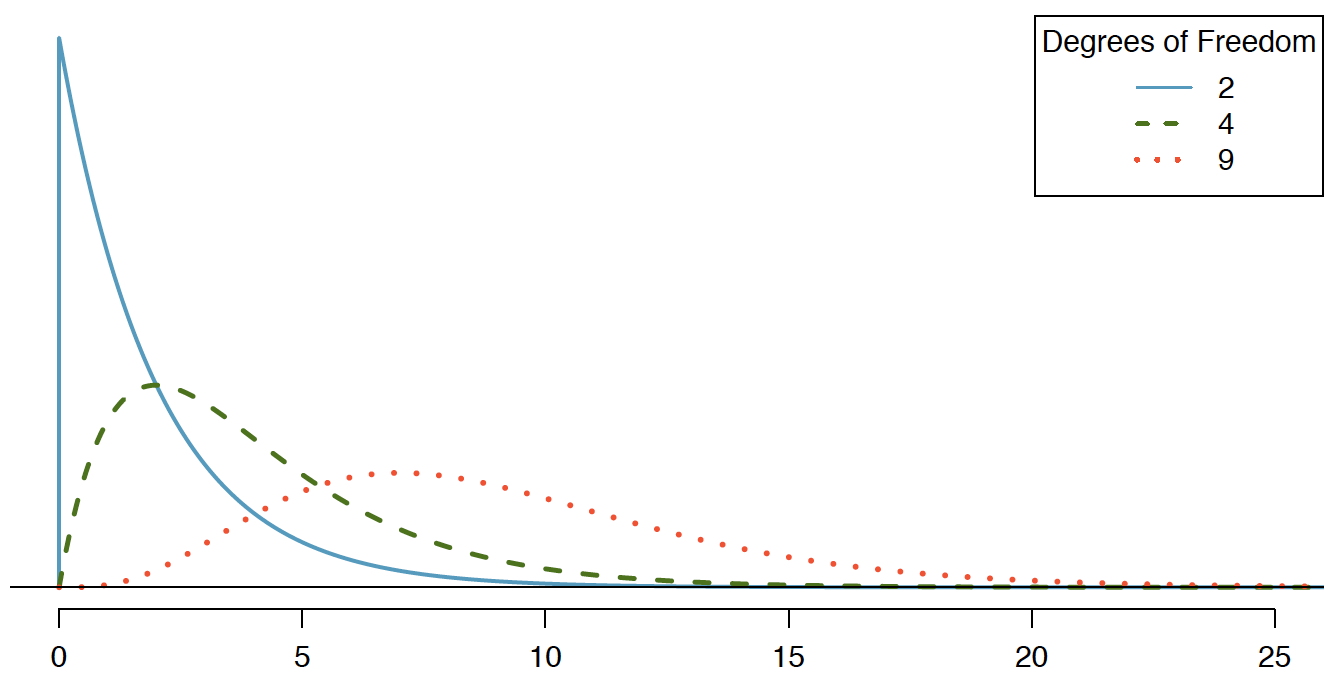
\includegraphics[width=0.8\textwidth]{figure/chi.png}
\end{center}

\end{frame}
%------------------------------------------------------------------------------


%------------------------------------------------------------------------------
\begin{frame}[fragile]
\frametitle{p-values}
The $p$-value is the \blue{area to the right} of the test statistic.  Use p.412:
\begin{center}
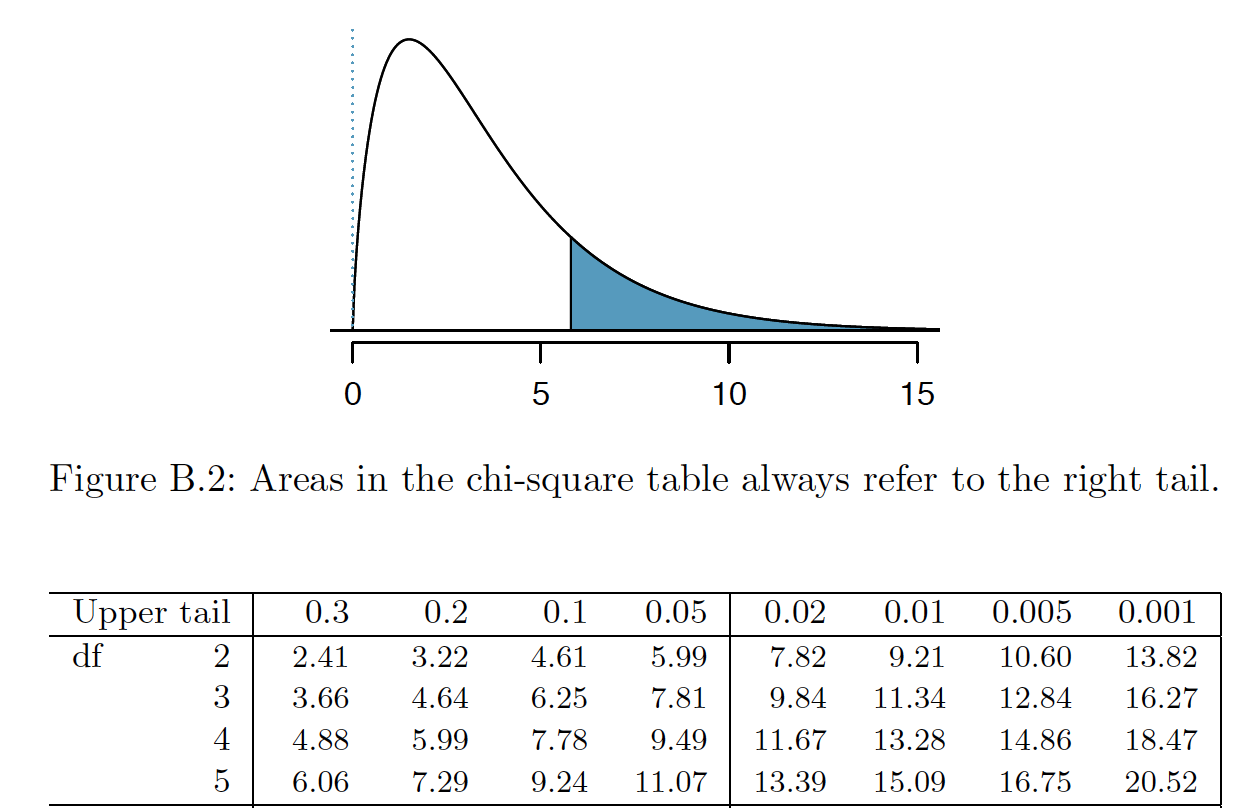
\includegraphics[width=0.8\textwidth]{figure/table.png}
\end{center}
%
% Comment this
%
\pause In our case, $df=k-1=3$, and $\chi^2=5.89$, which is in between $(4.64, 6.25)$, so p-value is in between $(0.1, 0.2)$.  Not overwhelming evidence against $H_0$.

\end{frame}
%------------------------------------------------------------------------------


%------------------------------------------------------------------------------
\begin{frame}[fragile]
\frametitle{Hypothetical Scenarios}
Say we have two hypothetical scenarios of observed counts:
\begin{center}
\begin{tabular}{l||cccc|c}
Race & White & Black & Hispanic & Other & Total \\ 
\hline
Expected Counts & 198 & 19.25 & 33 & 24.75 & 275\\ 
Observed Counts &  &  &  &  & 275 \\ 
\end{tabular}
\end{center}

%
% Comment this
%
%\pause 
\begin{itemize}
\item For all 4 groups, say observed = expected, then
\[
\chi^2 = 0 + 0 + 0 + 0 = 0
% Z_i^2=\frac{(\mbox{observed count}_i - \mbox{expected count}_i)^2}{\mbox{expected count}_i} = 0
\]
hence p-value = 1.
\pause\item Say we observed 275 others and 0 for the rest, then 
\[
\chi^2 = 2786.11 + 84.46 + 189.57 + 12588.11 = 15648.25
%c((0-198)^2/sqrt(198), (0-19.25)^2/sqrt(19.25), (0-33)^2/sqrt(33), (275-24.75)^2/sqrt(24.75))
\]
hence p-value = 0.
\end{itemize}

\end{frame}
%------------------------------------------------------------------------------


%------------------------------------------------------------------------------
\begin{frame}[fragile]
\frametitle{Assumptions for Chi-Square Test}
%
% Comment this
%
\begin{enumerate}
\item \blue{Independence}:  Each case is independent of the other
\pause\item \blue{Sample size}:  Similarly like with proportions, we need at least 5 cases in each scenario (each cell in the table)
\pause\item \blue{Degrees of freedom}:  We need at least $df=2$, i.e. $k\geq 3$
\end{enumerate}
\end{frame}
%------------------------------------------------------------------------------


%------------------------------------------------------------------------------
\begin{frame}[fragile]
\frametitle{Next Time}
We look at \blue{chi-square tests for two-way tables} to test for \blue{independence}.  i.e. are two variables independent from each other?

\end{frame}
%------------------------------------------------------------------------------


\end{document}










